\subsection{Sample Application of Formal and Insight Model}

We provide small case in \autoref{fig:wealth-weighted} to illustrate how both models can be applied in quantifying knowledge wealth. In this example, we will focus on the notion using bag of properties with outgoing direction of link to quantify the wealth.

\begin{figure}[!h]
    \centering
    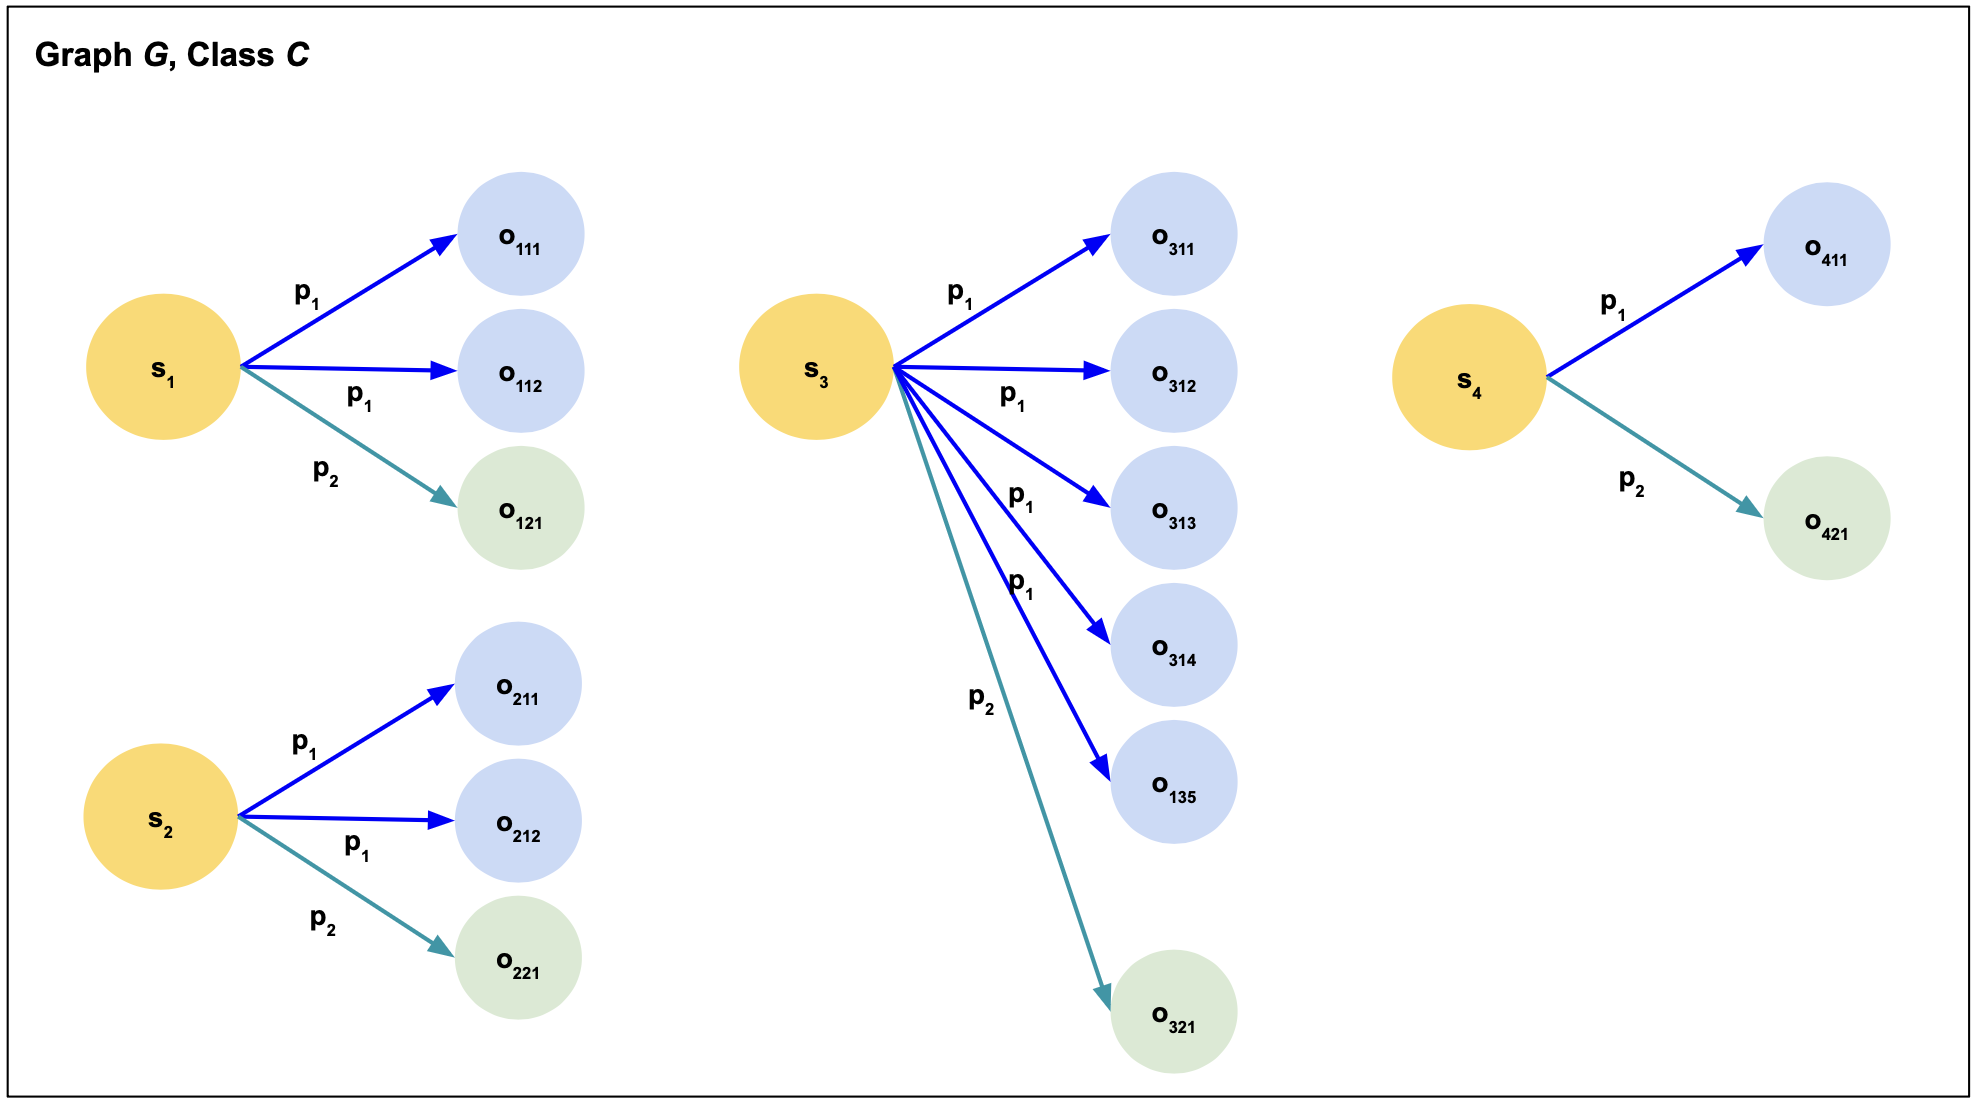
\includegraphics[scale=.3]{Wealth Weighted}
    \caption{Sample knowledge graph \(G\) that contains class \(C\) with 4 entities} \label{fig:wealth-weighted}
\end{figure}

A graph \(G\) has a class \(C\), which consists of 4 entities \(s_1\), \(s_2\), \(s_3\), and \(s_4\). Using bag of properties and outgoing link direction, the walth of entity \(s_1\), \(s_2\), \(s_3\), and \(s_4\) are 3, 3, 6, and 2 respectively. \autoref{tab:sample statistical summary} shows some statistical summary that describe the wealth of class \(C\).

\begin{center}
    \small
    \begin{threeparttable}
    \caption{Statistical Summary of Wealth of Class \(C\)}
    \label{tab:sample statistical summary}
    \begin{tabular}{c | c c c c c c c} 
    
    \toprule
        Measure & Entity Count & Mean & Median & Mode & Minimum & Maximum & Gini \\ [0.5ex] 
    \midrule
        Value & 4 & 3.5 & 3 & 3 & 2 & 6 & 0.21 \\
        [0.5ex]
    \bottomrule
    \end{tabular}
    \begin{tablenotes}
        \footnotesize
        \item{This table shows some statistical measures to quantify the wealth of class \(C\).}
    \end{tablenotes}
    \end{threeparttable}
\end{center}

In addition, Lorenz curve for wealth of entities in class \(C\) is shown in \autoref{fig:sample-lorenz}.

\begin{figure}[!h]
    \centering
    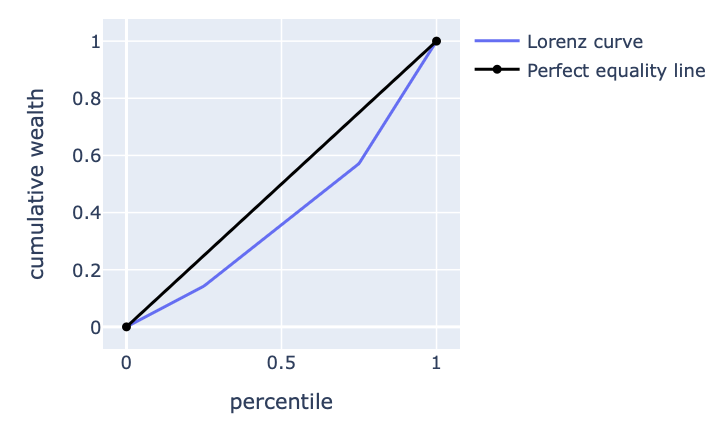
\includegraphics[scale=0.8]{Sample Lorenz Curve}
    \caption{Lorenz curve of class \(C\)} \label{fig:sample-lorenz}
\end{figure}